\documentclass{sig-alternate}
\usepackage{verbatim}
\usepackage{array}
\usepackage{caption}
\usepackage{subcaption}
\usepackage{amsmath}

\newtheorem{definition}{Definition}
\begin{document}

\numberofauthors{2}

%\author{[Blind]}
%\author{
%Craig Willis, Miles Efron, and Garrick Sherman \\
%     \affaddr{Graduate School of Library and Information Science}\\
%       \affaddr{University of Illinois at Urbana-Champaign}\\
%       \email{\{willis8, mefron, gsherma2\}@illinois.edu}
%}
\conferenceinfo{SIGIR}{'2016 Pisa, Italy}

\title{Detecting large-scale events in news corpora}

\maketitle
\begin{abstract}
Retrospective event detection is the task of identifying events in time-stamped corpora. In this short paper, we present a simple unsupervised method for identifying large-scale events in a news corpus based on feature temporal mutual information ($I_t$) and non-negative matrix factorization (NMF). We introduce a preliminary test collection and evaluation methodology that can be used for future comparative research. We compare our method to an approach based on latent Dirichlet allocation (LDA) to better understand key differences between events and topics.

\end{abstract}

% A category with the (minimum) three required fields
\category{H.3.3}{Information Search and Retrieval}{}

%\terms{}
%\keywords{Event detection}

\section{Introduction}

Imagine a journalist constructing a `year in review' article or a Wikipedia editor creating a page summarizing a list of important events that occurred during a particular year\footnote{e.g., https://en.wikipedia.org/wiki/1988\#Events}. Given a corpus of news articles (or other timestamped collection), it should be possible to show her a list of major events that were reported during the time period to facilitate the creation or validation of these pages. Such a system might rank the events by importance, provide estimated dates of event occurrence, and a ranking of candidate Wikipedia pages or articles that describe the associated event. 

In this short paper, we present a novel method for retrospective event identification in news corpora based on temporal mutual information \cite{Teng2008} and non-negative matrix factorization \cite{Lee2001}, which we call TMINMF. We also introduce a preliminary test collection and evaluation methodology based on Wikipedia that can be used for future comparative research.  As far as we know, we are the first to propose a method for comparative evaluation in this type of retrospective event identification task.

Following \cite{Weng2011}, we compare the results of our method to an LDA baseline. We find the TMINMF model is significantly better than the LDA model based on mean reciprocal rank (MRR) of events identified by the two models (two-sided t-test, $p < 0.001$) as well as the proportion of true events identified by the two models (Binomial proportion test, $p < 0.01$).

This short paper is organized as follows. In Section 2 we review the concept of an \emph{event} followed by a summary of related work in Section 3. In Sections 4 and 5 we introduce our model and the LDA baseline. Section 6 describes the evaluation methodology and test collection. Section 7 summarizes the results followed by conclusions and next steps in Section 8.

\section{What is an event?}

The concepts of `event detection' or `event extraction' are common in the information retrieval and natural language processing literature. In this paper, we are concerned with the identification of large-scale events as reported in historical news corpora.   Examples of large-scale events include major elections, natural disasters, political revolutions, wars, and other acts of violence.


\section{Related Work}

Recent studies in retrospective event identification apply feature-centric models \cite{Yi, Fung2005, Chen2009, Teng2008, Weng2011} that first identify interesting terms (or features) which are subsequently grouped or combined to represent events. 

For example, Fung et al \cite{Fung2005} identify temporally interesting features using a series of binomial distributions. The terms are subsequently combined  into events using a cost-minimization approach that balances the similarity of the temporal distributions of terms and the co-occurrence of terms in documents. 

He, Chang and Lim \cite{He2007} use spectral analysis to identify interesting features in text corpora. Features are grouped into events using a cost-minimization approach that combines the similarity of the temporal distributions using KL divergence and co-occurrence of terms in documents. 

Weng and Lee \cite{Weng2011} use wavelet analysis to identify interesting features which are used to construct a graph with terms as nodes and the cross-correlation of term time-series as edge weights. They apply a graph partitioning algorithm to identify events as sets of connected terms. 

Also related to the current study is research in latent semantic analysis (LSA) \cite{Deerwester1990, Hofmann1999} and topic modeling \cite{Blei2003}.  Event models can be seen as temporally-constrained topic models. Our approach is akin to the factor-based LSA, but we anticipate expanding this work to a generative probabilistic framework in the future.  




\section{Event detection model (TMINMF)}	

Each of the feature-centric models described above includes two basic steps. The first is to identify terms or features that are indicative of an event in the corpus (signals), generally using time-series methods. The second is to combine terms generated by the same underlying event into event models.  This is usually done by balancing temporal similarity (e.g., correlation of term time series) with term co-occurrence in documents.

In this study, we identify temporally interesting terms using the first-order autocorrelation (ACF) of the term time series \cite{Jones2007}. We then calculate the temporal mutual information between the top $k$ terms based on ACF and apply non-negative matrix factorization (NMF) to identify latent factors. We interpret the resulting factors as events. The basic process is defined as follows:

First, we construct a temporal index from the document collection that consists of time series for each term in the vocabulary at a particular interval (e.g., hour, day, week):
\begin{definition}
 \text{ \normalfont Term time series. }
 The time series of a term f is defined as the sequence:
\[
y_f = [y_f(1), y_f(2), ..., y_f(T)],
\]
where each element $y_f(t)$ is a measure of term f at time t. For this paper, we use the simple document frequency:
\[
	y_f(t) = DF_f(t)
\]
where $DF_f(t)$ is the number of documents containing term f at time t.
\end{definition}

Next, for each term in the vocabulary, we calculate the first-order autocorrelation ($\rho$) of the time series. 
\begin{definition}
 \text{ \normalfont First order autocorrelation. }
 Given 
\[
\rho = \dfrac{\sum_{i=1}^{N-1} (y_t - \bar{y}_{(1)})(y_{t+1} - \bar{y}_{(2)})}{ \big [ \sum_{i=1}^{N-1}  (y_t - \bar{y}_{(1)})^2 \big ] ^{1/2} \big [\sum_{i=1}^{N-1} (y_{t+1} - \bar{y}_{(2)})^2 \big ]^{1/2}}
\]
\end{definition}

As noted by \cite{Jones2007}, terms with high temporal dependency will have very high (1) or very low (-1) $\rho$.  For this short paper, we consider only the top $k$ terms based on ACF, where $k$ is chosen heuristically.

For the top $k$ terms, we calculate the temporal mutual information $I_t(x;y \vert t)$ between term pairs \cite{Teng2008}. 

\begin{definition}
 \text{ \normalfont Temporal mutual information. }
Given a timestamp $t$ and pair of terms $x$ and $y$, the temporal mutual information between $x$ and $y$ in $t$ is defined by:
\[
I_t(x;y \vert t) = p(x,y \vert t) \log \dfrac{p(x,y \vert t)}{p(x \vert t) p(y \vert t)}
\]
\end{definition}

In this study, $I_t(x;y \vert t)$ is calculated independently for each interval.

Finally, we construct a symmetric matrix of the maximum $I_t$ between terms and apply NMF \cite{Lee2001} to identify latent factors. 
\begin{definition}
 \text{ \normalfont Non-negative matrix factorization.}
 Given a non-negative matrix $V$, NMF finds matrix factors $W$ and $H$ such that:
\[
V \approx WH
\]
\end{definition}

We interpret the matrix $W$ as latent event models, using the assigned weights as term weights. We select the top $N$ factors based on the sum of the factor-term weights. The resulting event models are evaluated as described in Section 6.

\section{Baseline LDA model}

Most previous treatments of this task offer evaluation through `eyeballing' the quality of generated event models. Only \cite{Weng2011} compares their  method to an older baseline -- LDA.  However, while \cite{Weng2011} does offer comparative evaluation, the evaluation is again heuristic. Our goal in bringing LDA into this analysis is to allow quantitative assessment of the quality of TMINMF as compared to models generated by the well-studied LDA method. For details on the LDA model itself, the reader is directed to \cite{Blei2003}.

There is a relationship between event detection and topic modeling. Some topics are likely generated by events, particularly in news corpora.  The problem is how to identify them from the resulting set of topic models.

One approach is to consider LDA topics ranked by the first order autocorrelation (ACF) of the topic time-series. The time series of a topic $m$ is defined as the sequence:
\[
y_m = [y_m(1), y_m(2), ..., y_m(T)],
\]
where each element $y_m(t)$ is a measure of the topic $m$ at time $t$. For this paper, we use the sum of the document-topic probabilities for all document published at time $t$:
\[
	y_m(t) = \sum_{d \in D} p(m \vert d, t)
\]

We then calculate the ACF of each topic time series and rank topics by ACF, selecting the top $N$ topics for evaluation.  We hypothesize that topics with high ACF values are more likely to represent events.  The main difference between the LDA baseline and the TMINMF model described in Section 4 is that the TMINMF starts with a subset of terms with strong temporal signals, whereas the LDA method constructs topics from the entire vocabulary. Using the ACF approach, we look for temporal signals in the topic distributions over time. We compare the two approaches as described in the next section.


\begin{table*}[!htbp]
\scriptsize
\begin{tabular}{| l | p{1cm} | p{8cm} | p{6cm} | } \hline
{\bf ID} & {\bf Date} &  {\bf Description}  & {\bf Wikipedia URL} \\ \hline
19 & Mar 11 & Terrorists execute simultaneous attacks, with bombs in 4 rush-hour trains in Madrid, killing 191 people.	&  2004\_Madrid\_train\_bombings \\ \hline
42 & June 28 & The U.S. led coalition occupying Iraq transfers sovereignty to an Iraqi Interim Government.	& Iraqi\_sovereignty \\ \hline
57 & Sept 1 & Chechen terrorists take 1,128 people hostage, mostly children, in a school in the Beslan school hostage crisis. & Beslan\_school\_siege \\ \hline
76 & Nov 2 & United States presidential election, 2004: Republican incumbent President George W. Bush is declared the winner over his Democratic challenger, U.S. Senator John F. Kerry, in a close election. & United\_States\_presidential\_election,\_2004 \\ \hline
91 & Dec 26 & One of the worst natural disasters in recorded history hits Southeast Asia, when the strongest earthquake in 40 years, measuring 9.3 on the Richter scale, hits the entire Indian Ocean region. & 2004\_Indian\_Ocean\_earthquake\_and\_tsunami \\ \hline
\end{tabular}
\caption{Example entries from the known-events list (Wikipedia 2004)}
\label{table.knownevents}
\end{table*}

\section{Evaluation}

In this section, we outline a preliminary methodology and test collection that can be used for future comparative evaluation. A primary concern in the evaluation of feature-centric event detection is how effective the model is at identifying true events in the corpus. For this short paper, we propose an evaluation methodology based on Wikipedia and the pooled results of the systems under comparison.

We hypothesize that high-quality event models will serve as effective queries against external corpora, such as Wikipedia. Each event model is, in essence, a language model describing an event and as such fit naturally into a KL-divergence ranking framework. For evaluation, we use the candidate event models as queries against an indexed copy of Wikipedia, returning the top $j$ pages. The retrieval system is Indri with Dirichlet smoothing ($\mu=2500$). 
Before evaluation, each system generates a set of $N$ candidate event models from a news corpus (e.g., New York Times or Associate Press). Each event model contains a list of $k$ terms with associated weights, which are used as a query against Wikipedia returning the top $j$ pages (represented as URLs).

To develop a ground-truth of \emph{known-events}, we start with events listed in the Wikipedia `year' pages for the period of the document collection\footnote{https://en.wikipedia.org/wiki/2004\#Events}. The known-event list contains the event description, dates, and associated Wikipedia URL. We then pool the URLs returned by the two systems, which are manually reviewed to identify any missing events from the known-events list.  At the end of this process, we have a ground-truth of unique known-events represented as Wikipedia page URLs, based on a combination of the Wikipedia year pages and the pooled results from the systems.  

For each of the top $N$ candidate events, we compare the systems based on (1) the mean reciprocal rank (MRR) of the first unseen known-event in the list of Wikipedia URLs and (2) the proportion of known events identified in the top $N$ candidate events at each depth.  This approach allows us to compare systems without requiring qualitative human assessment of individual event models.

\subsection{Test metrics}

To compare system effectiveness, we need metrics that capture event model quality (e.g., returning the `best' Wikipedia page for an event) and event coverage (i.e., identifying the most unique known events) while addressing the problem of redundancy. We've selected two separate metrics.  

A variation of mean reciprocal rank (MRR) is used to capture event model quality. We calculate the rank of the first known-event URL returned by the system for each candidate event. The known-event URLs can only be considered once per system. Therefore, if two candidate events return the same known-event URL, it is only counted for the first candidate event.
\[
MRR = \dfrac{1}{N} \sum_{i=1}^{N} \dfrac{1}{rank_i}
\]
Next, we calculate the simple proportion of unique Wikipedia URLs returned by each system that are found in the known events list.
\[
p = \dfrac{\vert \text{ Unique URLs returned} \cap \text{Known events list} \vert}{\vert \text{Unique URLs returned} \vert}
\]

We compare MRR using a two-sided t-test and the $p$ using a two-sided Binomial proportion test.

\subsection{Test collection}
News articles from the year 2004 in the New York Times Annotated Corpus \cite{Sandhaus2008} are used for evaluation. Only articles found in Section A (available via document metadata) are considered and summary articles are ignored. Stopwords are removed using the standard Indri list. The resulting collection consists of 25,689 documents.

The ``known-events'' list is constructed using the process described in the previous section based on the ``Events'' section of the 2004 Wikipedia year page\footnote{https://en.wikipedia.org/wiki/2004\#Events} and the top $N=50$ candidate events from the two systems.  The final ``known-events'' list contains 126 unique events represented by Wikipedia URLs. Of these events, 95 are from the Wikipedia year page and the remaining 31 were added based on the pooled system results.  Selected entries from the known-events list are presented in Table \ref{table.knownevents}.  The indexed copy of Wikipedia is from 09/01/2015.

\section{Results}
\begin{figure}
\centering
\begin{subfigure}{.25\textwidth}
  \centering
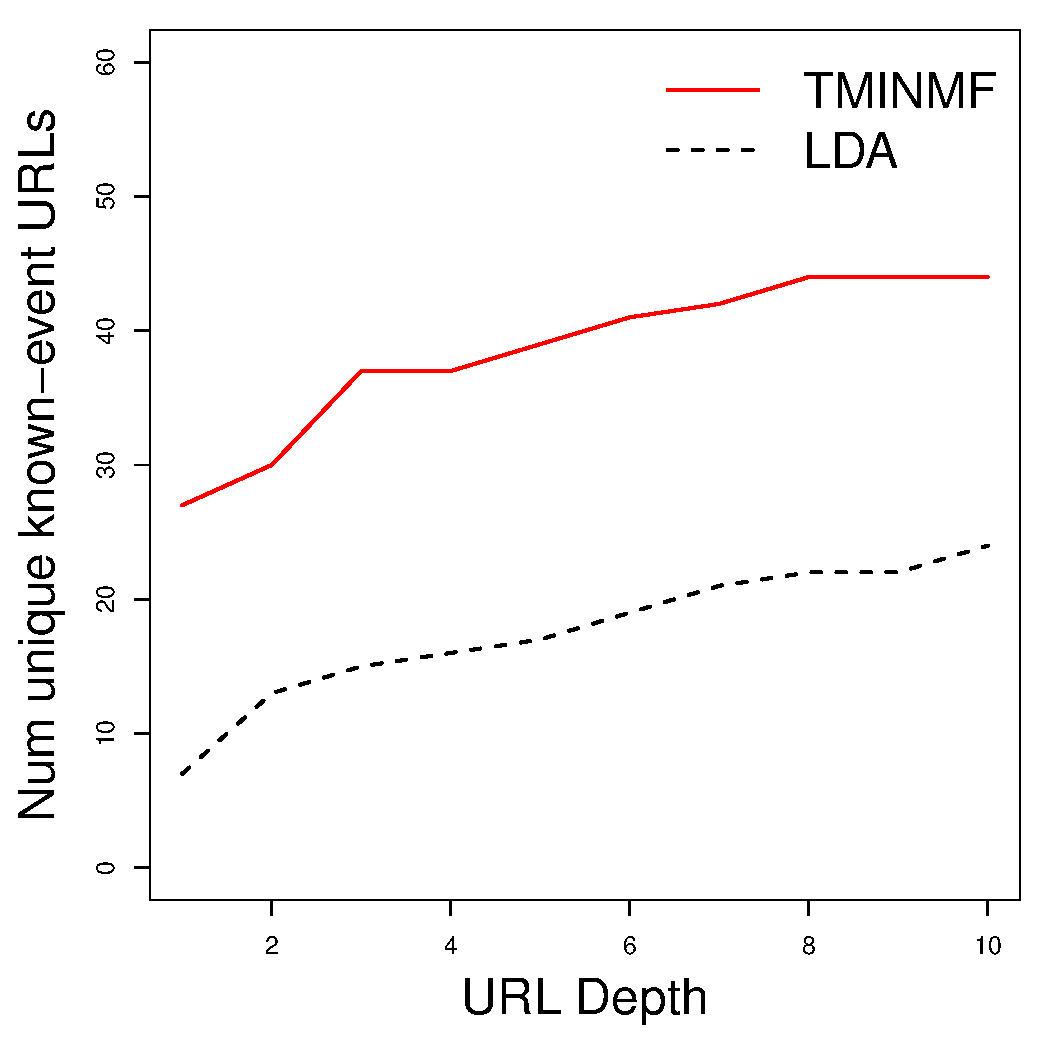
\includegraphics[width=4cm]{plots/events_at_depth.pdf}
\end{subfigure}%
\begin{subfigure}{.25\textwidth}
  \centering
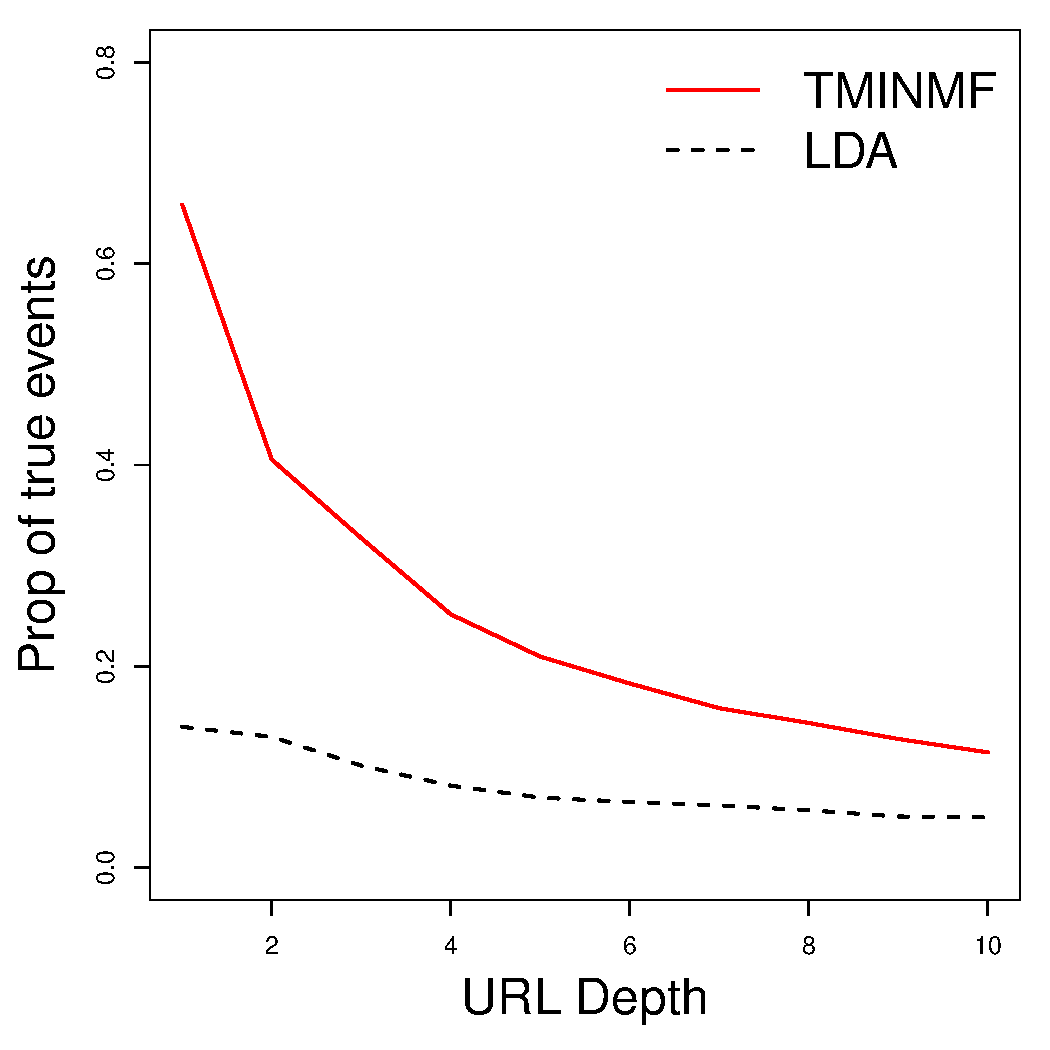
\includegraphics[width=4cm]{plots/prop_at_depth}
\end{subfigure}
\caption{(a) number of unique known-event URLs at each depth, (b) proportion of unique known-event URLs at each depth}
\label{fig.eventdist}
\end{figure}


\begin{table}
\scriptsize
\begin{tabular}{| p{0.2cm} | p{3.5cm} | p{3.5cm} | } \hline
{\bf ID } & {\bf TMINMF} & {\bf LDA } \\ \hline
1 & wesley(0.075) clark(0.074) dean(0.055) primary(0.052) howard(0.05) edwards(0.05) kerry(0.049) & 
edwards(0.048) dean(0.048) campaign(0.043) dr(0.034) kerry(0.025) candidate(0.024) s(0.018)   \\ \hline
2 & taguba(0.036) soldier(0.035) detainee(0.03) prisoner(0.029) karpinski(0.029) ricardo(0.028) fay(0.028)   &
prisoner(0.034) military(0.033) abuse(0.026) detainee(0.025) interrogate(0.023) iraq(0.023) prison(0.021)  \\ \hline
3 & poll(0.181) voter(0.131) politics(0.131) bush(0.112) election(0.11) campaign(0.102) vote(0.098)  &
kerry(0.135) bush(0.071) campaign(0.046) s(0.038) president(0.028) john(0.018) senator(0.016) \\ \hline
4 & port(0.044) au(0.04) aristide(0.038) prince(0.033) philippe(0.032) rebel(0.03) haitien(0.028) &
haiti(0.049) aristide(0.037) government(0.022) cuba(0.018) s(0.015) president(0.014) rebel(0.013)  \\ \hline
5 & sadr(0.05) moktada(0.044) baghdad(0.042) sunni(0.039) militia(0.037) falluja(0.036) occupation(0.03)  &
vote(0.077) election(0.059) voter(0.057) percent(0.03) poll(0.027) ballot(0.022) party(0.021) \\ \hline
\end{tabular}
\caption{Top 5 events detected by TMINMF and LDA methods}
\label{table.top5}
\end{table}

The TMINMF model was run using a daily interval with the top 1000 terms based on ACF and $k=50$ factors for NMF. The LDA model was run using the Mallet implementation with $T=100$ topics, an interval of 10 for hyperparameter optimization, and all other default values. Only the top $N=50$ LDA topics were considered as events for evaluation\footnote{This is done to help eliminate the more general LDA topics, i.e., those containing common words/stopwords} based on topic time series ACF.

The top 5 events from both the TMINMF and LDA methods are presented in Table \ref{table.top5}. Outwardly, the models look similar and would be difficult to compare qualitatively.  Figure \ref{fig.eventdist} compares the TMINMF and LDA approaches.  The first graph (a) shows the number of unique known-event URLs returned by the two systems at each depth ($1 \le d \le 10$).  The second graph (b) shows the proportion of unique URLs that are found in the known-item list  at each depth.

Finally, we compare the two systems using the MRR of the first known-item URL for each candidate event and the proportion of known events identified, as described in Section 6.1.  The MRR of the TMINMF and LDA models is 0.4965 and 0.160 respectively. The means are not equal based on a two-sided t-test ($p < 0.001$).   The proportions at a depth of 1,   $p_{TMINMF}=27/41=0.6585$ and $p_{LDA}=7/50=0.1400$.  At a depth of 5, the proportion of events is $p_{TMINMF}=39/186=0.2097$ and $p_{LDA}=17/244=0.0697$. Using a two-sided binomial proportion test, in both cases the proportions are not equal ($p < 0.01$).


\section{Conclusions}

Based on these results, we can see that the TMINMF model is consistently more effective at identifying known-events than the ACF-ranked LDA topics.  From this we can conclude that the TMINMF model is more effective both in terms of event coverage (i.e., more unique known events were returned) and in event model quality (i.e., the event models serve as better queries to Wikipedia).  

The TMINMF approach has several strengths. First, it is principled, relying on a well-known methods to measure term associations (mutual information) and factor analysis (NMF). Second, by using NMF terms can be assigned to multiple event models (similar to LDA).  Third, it has a natural way of weighting terms based on the assigned factor weights. While this is also true with LDA, it is not the case with previous models such as \cite{He2007}.  

This short paper has introduced a simple and effective method for retrospective event detection in news corpora. Previous research in this area has relied on predominantly on isolated qualitative evaluation to assess model effectiveness. We have also introduced a preliminary evaluation methodology that can be used for future comparative evaluations. Using this evaluation methodology, we demonstrate that our simple model is effective and outperforms an LDA-based approach. 

Future work: We plan to explore event models in the generative probabilistic framework. We will expand the current method to include estimation of event dates and ranking events by importance. We will expand and refine the evaluation methodology. We plan to evaluate this method using a larger corpus -- for example, the LDC NYT collection covers the years 1987-2007.


\section{Acknowledgments}
This work was supported in part by the US National Science Foundation under Grant No. [blind]. Any opinions, findings, conclusions, or recommendations expressed are those of the authors and do not necessarily reflect the views of the National Science Foundation.


\bibliographystyle{abbrv}
\bibliography{eventdetection}  




\end{document}
